\documentclass[11pt,a4paper]{article}
\usepackage[margin=2.5cm]{geometry}
\usepackage[T1]{fontenc}
\usepackage{lmodern}
\usepackage{microtype}
\usepackage{amsmath,amssymb,bm}
\usepackage{graphicx}
\usepackage{xcolor}
\usepackage{caption}
\captionsetup{font=small,labelfont=bf}
\usepackage[breaklinks=true]{hyperref}
\hypersetup{colorlinks=true,linkcolor=blue!60!black,urlcolor=blue!55!black,
  citecolor=blue!60!black}

\title{\textbf{Chirality-induced spin selectivity as a spin gate on
mitochondrial superoxide production:\\ a radical-pair model}}
\author{O.~Kirichenko\\[2pt]\small Independent Researcher \quad$\cdot$\quad
  \href{mailto:urevich55@gmail.com}{urevich55@gmail.com}}
\date{\today}

\begin{document}
\maketitle

\begin{abstract}
\noindent
The inner mitochondrial membrane sustains an electric field of
$\sim\!3.5\times10^{7}$~V/m, and electrons traverse a chain of chiral
cofactors (flavin, Fe--S clusters, hemes) embedded in helical proteins.
Chirality-induced spin selectivity (CISS) therefore spin-filters the
respiratory electron before it can leak to molecular oxygen. We model the
resulting $\{\text{flavin semiquinone}^{\bullet-}\!\cdots\text{O}_2^{\bullet-}\}$
radical pair with a Liouville--von~Neumann equation including Zeeman and
hyperfine interactions and Haberkorn spin-selective recombination, and we
represent the CISS electron transfer as a coherent spin rotation of a
singlet precursor. The model predicts that (i)~CISS \emph{raises} the
triplet (superoxide-escape) yield---from $8\%$ at zero polarization to
$17\%$ at $70\%$ polarization in our reference parameters---and (ii)~a
weak static magnetic field of order the flavin hyperfine scale
($\sim\!1$~mT) modulates that yield by a few percent, in the direction and
magnitude reported experimentally by Usselman et~al. The framework yields
three falsifiable predictions distinguishing a CISS-controlled radical
pair from a chirality-independent one. No exotic physics is invoked: every
ingredient (the field, CISS, the flavin--oxygen radical pair, and its
measured magnetic sensitivity) is independently established.
\end{abstract}

\section{Motivation}
Reactive oxygen species (ROS), principally superoxide $\text{O}_2^{\bullet-}$,
are unavoidable byproducts of oxidative phosphorylation and central to
redox signalling and ageing. Superoxide forms when an electron leaks from
a reduced cofactor---the flavin of Complex~I or the semiquinone of
Complex~III---to $\text{O}_2$. The nascent
$\{\text{D}^{\bullet+}\!\cdots\text{O}_2^{\bullet-}\}$ pair is a
\emph{radical pair}: its overall electron-spin state (singlet $S$ or
triplet $T$) is conserved on the nanosecond timescale of the encounter
and selects the fate of the pair---singlet back-transfer (to
$\text{H}_2\text{O}_2$ or the reduced donor) versus triplet escape (to
free superoxide)~\cite{steiner,hore}.

Two facts make this a spin-chemistry problem rather than a metaphor.
First, the respiratory cofactors are chiral and helically arranged, so the
transferred electron is spin-polarized by chirality-induced spin
selectivity (CISS), an effect measured at room temperature with
polarizations of tens of percent through DNA and
$\alpha$-helices~\cite{naaman,waldeck}. Second, Usselman et~al. showed that
static magnetic fields of $\sim\!1$--$3$~mT shift the cellular
$\text{O}_2^{\bullet-}/\text{H}_2\text{O}_2$ ratio~\cite{usselman}, the
hallmark of a radical-pair mechanism operating in living mitochondria.
Here we ask, quantitatively: if CISS sets the initial spin state of the
flavin--oxygen radical pair, how does superoxide output depend on the CISS
polarization and on an applied field?

\section{Model}
\subsection{Spin Hamiltonian}
We take two electron spins---$A$ (donor semiquinone) and $B$
($\text{O}_2^{\bullet-}$)---and one spin-$\tfrac12$ nucleus hyperfine-coupled
to $A$ (the flavin; superoxide is essentially hyperfine-free). In angular
frequency units,
\begin{equation}
  H = \gamma_e B\,(S_{Az}+S_{Bz})
    + a\,\bm{S}_A\!\cdot\!\bm{I},
\end{equation}
with electron gyromagnetic ratio
$\gamma_e = 1.76\times10^{8}\,\text{rad\,s}^{-1}\text{mT}^{-1}$ ($g\simeq2$)
and an effective flavin hyperfine coupling $a = \gamma_e\times1.0$~mT.

\subsection{Spin-selective recombination}
Reaction is described by the Haberkorn master equation~\cite{haberkorn},
\begin{equation}
  \dot\rho = -\tfrac{i}{\hbar}[H,\rho]
    - \tfrac{k_S}{2}\{P_S,\rho\}
    - \tfrac{k_T}{2}\{P_T,\rho\},
\end{equation}
where $P_S=\tfrac14-\bm{S}_A\!\cdot\!\bm{S}_B$ and $P_T=\mathbb{1}-P_S$ are
the singlet/triplet projectors and $k_S=10^{7}\,\text{s}^{-1}$,
$k_T=10^{6}\,\text{s}^{-1}$ are the channel rates (singlet back-transfer
faster than triplet escape). Reaction yields follow from the time integral
$\tilde\rho=\int_0^\infty\!\rho\,dt=-\mathcal{L}^{-1}\rho(0)$, with
$\mathcal{L}$ the Liouvillian superoperator, as
$\Phi_S=k_S\,\mathrm{Tr}[P_S\tilde\rho]$,
$\Phi_T=k_T\,\mathrm{Tr}[P_T\tilde\rho]$; superoxide escape corresponds to
$\Phi_T$.

\subsection{The CISS initial state}
A bonded electron transfer is born singlet. CISS rotates the transferred
electron's spin about the transfer axis; following the coherent treatment
of Fay and of Luo \& Hore~\cite{fay,luohore} we write
\begin{equation}
  \rho(0) = R_A(\varphi)\,\frac{P_S}{\mathrm{Tr}\,P_S}\,R_A^\dagger(\varphi),
  \qquad R_A(\varphi)=e^{-i\varphi S_{Ay}},\quad \sin\varphi = P,
\end{equation}
so that $P=0$ recovers the conventional singlet-born radical pair and
$P>0$ injects singlet--triplet coherence set by the CISS polarization.

\section{Results}
Figure~\ref{fig:ros} collects the three signatures of the model, each of
which doubles as a laboratory control.

\begin{itemize}
\item \textbf{(a) Chirality raises baseline superoxide.} At $B=0$,
  $\Phi_T$ rises from $8.2\%$ for the achiral control ($P=0$, dashed) to
  $10.2\%$ at $P=0.35$ and $17.4\%$ at $P=0.70$: the chirality-injected
  singlet--triplet coherence leaks population into the escaping triplet
  channel. The achiral curve is the reference a genuinely
  chirality-free leak site would produce.
\item \textbf{(b) Isotope test.} The low-field peak sits at
  $B_{\rm pk}\!\propto\!a$: the $^1$H flavin ($a=1.0$~mT) peaks at
  $B_{\rm pk}\!\approx\!0.23$~mT, and deuteration to $a=0.35$~mT shifts it
  to $\approx0.14$~mT. This is the standard radical-pair diagnostic and it
  fingerprints the flavin as the hyperfine partner.
\item \textbf{(c) Magnetic swing.} A weak field ($0\!\to\!1$~mT) changes
  $\Phi_T$ by a few percent absolute in every case---the low-field
  effect---matching the direction and magnitude of the measured
  mitochondrial ROS response to millitesla fields~\cite{usselman}. The
  swing is CISS-independent in size but rides on the CISS-set baseline.
\end{itemize}

\begin{figure}[t]
\centering
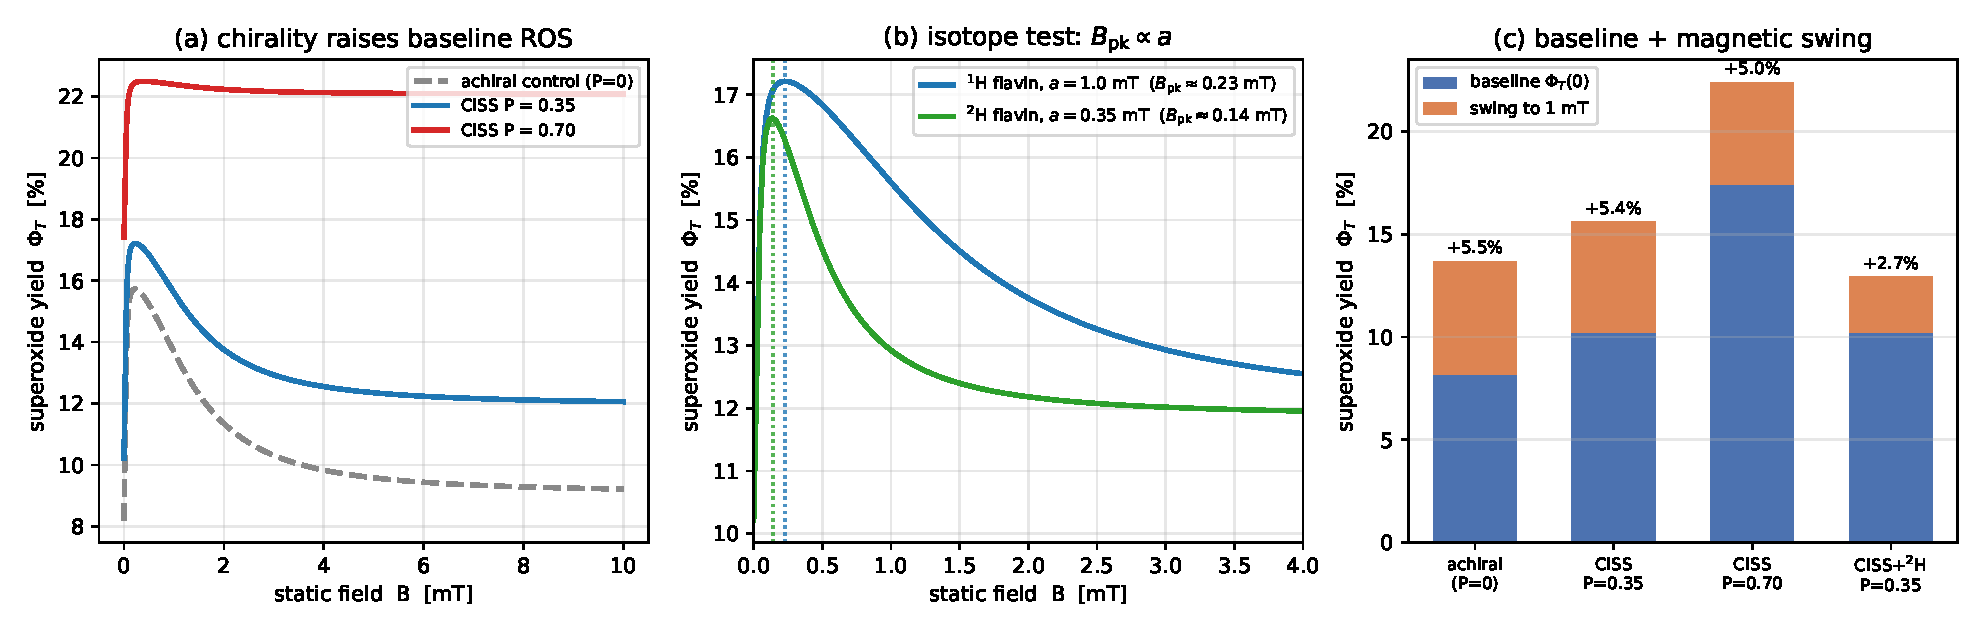
\includegraphics[width=\textwidth]{fig_ros_vs_B.pdf}
\caption{Superoxide (triplet) yield $\Phi_T$ of the flavin--oxygen radical
pair from the Liouville--Haberkorn model. \textbf{(a)} CISS polarization
raises baseline superoxide; the achiral control ($P=0$, dashed) is the
chirality-free reference. \textbf{(b)} Isotope test: the low-field peak
$B_{\rm pk}\propto a$ shifts under flavin deuteration ($^1$H vs $^2$H).
\textbf{(c)} Baseline yield (blue) plus its magnetic swing to $1$~mT
(orange) for each case. Every number is reproduced by
\texttt{ciss\_rpm\_model.py} / \texttt{ciss\_rpm\_figure.py}.}
\label{fig:ros}
\end{figure}

\section{Falsifiable predictions}
The CISS-controlled radical pair is distinguishable from a
chirality-independent one:
\begin{enumerate}
\item \textbf{Chirality knockout.} Racemizing or replacing the chiral
  scaffold of the leak site (a model electron-transfer construct with an
  achiral bridge) removes the CISS baseline shift and flattens the
  $P$-dependence, while leaving the intrinsic radical-pair low-field
  effect intact.
\item \textbf{Asymmetric field curve.} The $\Phi_T(B)$ curve carries a
  CISS-set asymmetry (its zero-field offset scales with $P$), absent in a
  purely singlet-born pair.
\item \textbf{Isotope test.} Deuterating the flavin lowers the effective
  hyperfine $a$ and shifts the low-field peak $B_{\rm pk}\propto a$
  (Fig.~\ref{fig:ros}b: $0.23\!\to\!0.14$~mT)---the standard radical-pair
  diagnostic---without changing the CISS baseline offset.
\end{enumerate}

\section{Scope and limitations}
This is a minimal two-electron/one-nucleus model; a quantitative fit to a
specific complex requires the full hyperfine tensor set of the flavin, the
$g$-anisotropy and fast spin relaxation of $\text{O}_2^{\bullet-}$, and the
in-situ recombination rates, none of which change the qualitative result.
The CISS polarization at the leak site is not yet measured and enters as a
parameter. The claim here is bounded and testable: chirality plus a weak
field jointly set superoxide output through a radical pair whose existence
and magnetic sensitivity are already established experimentally.

\begin{thebibliography}{99}\small
\bibitem{steiner} U.~E.~Steiner, T.~Ulrich, ``Magnetic field effects in
  chemical kinetics and related phenomena,'' Chem.\ Rev.\ \textbf{89}
  (1989) 51.
\bibitem{hore} P.~J.~Hore, H.~Mouritsen, ``The radical-pair mechanism of
  magnetoreception,'' Annu.\ Rev.\ Biophys.\ \textbf{45} (2016) 299.
\bibitem{naaman} R.~Naaman, Y.~Paltiel, D.~H.~Waldeck, ``Chiral molecules
  and the electron spin,'' Nat.\ Rev.\ Chem.\ \textbf{3} (2019) 250.
\bibitem{waldeck} B.~P.~Bloom, Y.~Paltiel, R.~Naaman, D.~H.~Waldeck,
  ``Chiral induced spin selectivity,'' Chem.\ Rev.\ \textbf{124} (2024)
  1950.
\bibitem{usselman} R.~J.~Usselman \emph{et al.}, ``The quantum biology of
  reactive oxygen species partitioning impacts cellular bioenergetics,''
  Sci.\ Rep.\ \textbf{6} (2016) 38543.
\bibitem{haberkorn} R.~Haberkorn, ``Density matrix description of
  spin-selective radical pair reactions,'' Mol.\ Phys.\ \textbf{32}
  (1976) 1491.
\bibitem{fay} T.~P.~Fay, ``Chirality-induced spin coherence in electron
  transfer reactions,'' J.\ Phys.\ Chem.\ Lett.\ \textbf{12} (2021) 1407.
\bibitem{luohore} J.~Luo, P.~J.~Hore, ``Chiral-induced spin selectivity in
  the formation and recombination of radical pairs,'' New J.\ Phys.\
  \textbf{23} (2021) 043032.
\end{thebibliography}

\vspace{4pt}
\noindent\footnotesize Code: \texttt{ciss\_rpm\_model.py} reproduces every
number and the figure (Liouville--von~Neumann propagation, 8-dimensional
spin space).
\end{document}
